\documentclass[a4paper]{article}

\usepackage[T1]{fontenc}
\usepackage{textcomp}
\usepackage[english]{babel}
\usepackage{hyperref}
\usepackage{amsmath, amssymb, amsthm}
% for \lightning
\usepackage{stmaryrd}
\usepackage{geometry}
\usepackage{tikz-cd}
% for \{mid,bottom,top}rule
\usepackage{booktabs}
% for MATLAB
\usepackage{matlab-prettifier}

\lstset{
	tabsize=4,
	style=Matlab-Pyglike,
	frame=single,
	numbers=left,
}

% Remove indentation globally
\setlength{\parindent}{0pt}
% Have blank lines between paragraphs
\usepackage[parfill]{parskip}

\hypersetup{
	colorlinks = true, % links instead of boxes
	urlcolor   = cyan, % external hyperlinks
	linkcolor  = blue, % internal links
	citecolor  = cyan   % citations
}

\newcommand{\R}{\mathbb{R}}
\newcommand{\C}{\mathbb{C}}
\newcommand{\Q}{\mathbb{Q}}
\newcommand{\N}{\mathbb{N}}
\newcommand{\A}{\mathbb{A}}
\newcommand{\Z}{\mathbb{Z}}

\renewcommand{\labelitemii}{$\circ$}
\renewcommand{\Im}{\operatorname{Im}}

\newcommand\numberthis{\addtocounter{equation}{1}\tag{\theequation}}

\newtheorem{theorem}{Theorem}[section]
\newtheorem{lemma}{Lemma}[section]

\theoremstyle{definition}
\newtheorem{definition}{Definition}[section]

\theoremstyle{definition}
\newtheorem{example}{Example}[section]

\theoremstyle{remark}
\newtheorem*{remark}{Remark}

\theoremstyle{definition}
\newtheorem{exercise}{Esercizio}[section]
\newtheorem*{exercise*}{Esercizio}

\title{Project Report: GMRES Method applied to PageRank}
\author{Francesco Minnocci}

\begin{document}
\maketitle
\section{Introduction to PageRank}
Developed at Google to model the problem of ranking pages on the World-Wide Web, the PageRank algorithm takes an adjacency matrix $H$ representing the graph associated to a
network (so that pages are nodes and links between pages are edges), and computes the
importance of each node as determined by the pages which point to it.

The assumption is that each page distributes its importance uniformly to its forward star: more precisely, if
 $$ d_i:=\sum_{i=1}^{n} h_{ij} ,$$
 the weight (or importance) of a node is defined as $$ w_j:=\sum_{i=1}^{n} w_i \frac{h_{ij}}{d_i} .$$

 This means that finding the weights corresponds to finding a left eigenvector $w^T$ relative to the eigenvalue $1$ for the matrix $D^{-1}H$, where $D=\operatorname{diag}(He)$: $$ w^T=w^T\left( D^{-1}H \right)
 .$$
 Existence of the solution is easily checked by computing $D^{-1}H\cdot e=e$, while in order to ensure positivity and uniqueness of the solution, we need to modify the model so
 that it satisfies the Perron-Frobenius theorem, which we state in the following form:
 \begin{theorem}
	 Let $A=(a_{ij})$ be a matrix with positive entries $a_{ij}>0$. Then, $A$ has a simple eigenvalue $\lambda=\rho(A)\geq 0$, and every other eigenvalue $\mu$ has absolute
	 value
	 $|\mu|<\rho(A)$. Moreover, there exists a left eigenvector $x$ and a right eigenvector $y$ which have positive entries, and they are unique up to scalar multiples.
 \end{theorem}
 We thus tweak our model by defining the following matrix, which satisfies the Perron-Frobenius theorem:
 $$ A=\gamma D^{-1}H+(1-\gamma)ev^T,~\gamma\in\left( 0,1 \right) ,\:v>0\text{ with }v^t e=1 .$$
 The parameter $\gamma$, known in the literature as \textit{damping factor}, determines what percentage of the weights is to distributed according to the original model, so
 that $(1-\gamma)$ determines
 how much is to be distributed according to the \textit{personalization vector} $v$. In this project, we will choose $v$ to be $e/n,$ which corresponds to choosing an uniform
 distribution across all nodes.
 As $A>0$ and $$Ae=\gamma D^{-1}He+(1-\gamma)ev^Te=\gamma e+(1-\gamma)e=e,$$ by Perron-Frobenius there exists a non-negative left eigenvector $w^T$ for the unique eigenvector of
 absolute value 1.
 While it is classical to solve this eigenvector problem with the Power Method \cite{bini}, we can rephrase it as a linear system: by asking that $w^t e=1$ and taking the
 transpose, we get:
 \begin{equation}\label{eq:linsys} (I-\gamma HD^{-1})w=\frac{1-\gamma}{n}e ,\end{equation}
 which is an invertible linear system as $\rho(HD^{-1})=1$ and $\gamma<1$.
\section{GMRES Method}
To solve \eqref{eq:linsys}, we are going to employ a Krylov method known as GMRES (Generalized Minimal RESidual). Krylov methods for linear systems are based on the observation
that, thanks to the Hamilton-Cayley theorem, we can compute the solution of an invertible $n\times n$ linear system $$Ax=b$$ as $$x=p(A)b,$$ for a polynomial $p(t)$ of degree at
most $n-1$. Since $n\gg0,$ we would like to find a lower degree polynomial $p_\ell$ such that $p_\ell(A)b$ is a good approximation of $x$.
With this is mind, we introduce the \textit{Krylov susbspace}
\begin{equation}\label{eq:krylov}
 \mathcal{K}_\ell(A,b):=\operatorname{span}{(b,Ab,\dots,A^{\ell-1}b)},
\end{equation}
so that the desired approximated solution lies in $\mathcal{K}_\ell$.

The GMRES method sets out to look for such solution as the vector with \textit{minimum residual} inside the Krylov subspace:
$$ x_\ell:=\arg\min\nolimits_{x\in\mathcal{K}_\ell}{\|Ax_\ell-b\|_2} .$$
In practice, this is achieved by solving the above least-squares problem through the Moore-Penrose pseudoinverse, appropriately restricting the solution to the order $\ell$ Krylov
susbpace in doing so (\cite{notes}, p. 53).

In order to build an iterative method based on Krylov subspaces, we need to determine a numerically well-conditioned basis of $\mathcal{K}_\ell$, for which we are going to use the Arnoldi
method, which iteratively finds an orthonormal basis for $\mathcal{K}_\ell$ by reothonormalizing at each iteration after computing the necessary matrix-vector product with $A$,
which in our project will be fast to compute (as $A$ will be sparse).
\section{Implementation}
Here is our MATLAB code which implements the GMRES method using the Arnoldi iteration. It takes in input the datum of the linear system and a tolerance value \texttt{eps}, used to
establish the convergence of the method. Its output contains the approximated solution \texttt{x}, the residual norm \texttt{res} relative to \texttt{x}, and a vector
\texttt{resvec} containing the residuals
at every iteration.
\begin{lstlisting}
function [x, res, it, resvec] = gmres_arnoldi(A, b, eps)
	n = size(A, 1);
	maxit = 100;
	beta = norm(b);
	resvec = [beta];
	v1 = b/beta;
	V = zeros(n, maxit);
	H = zeros(maxit, maxit);
	V(:, 1) = v1;

	% Arnoldi iteration
	conv = 0;
	j = 0;
	while (conv == 0 && j < maxit)
		j = j + 1;
		w = A * V(:, j);

		% Ortogonalization of A*v_j
		H(1:j, j) = V(:, 1:j)' * w;
		w = w - V(:,1:j) * H(1:j, j);

		% Normalization of the orthogonalized vector
		H(j + 1, j) = norm(w);
		V(:, j + 1) = w / H(j + 1, j);

		% Solving the least-squares problem
		e1 = zeros(j + 1, 1);
		e1(1) = beta;
		y = H(1:j+1,1:j) \ e1;

		% Computing the residual norm
		res = norm(H(1:j+1,1:j) * y - e1);
		resvec = [resvec; res];

		% Convergence check
		if res < eps
			x = V(:,1:j) * y;
			conv = 1;
			it = j;
		end
	end
end
\end{lstlisting}
We then tested the method on a dataset coming from the \texttt{coAuthorsDBLP} problem, available at \href{https://sparse.tamu.edu/DIMACS10/coAuthorsDBLP}{sparse.tamu.edu}. Here is
the script which was written to test the above method; the code uses 4 different values for the damping factor ($\gamma = 0.5, 0.7, 0.85, 0.99$), and a tolerance level of $10^{-8}$.
The script also plots the convergence information (residuals against number of iterations) for each value of $\gamma$, which we will discuss later.
\begin{lstlisting}
% Load the matrix
load coAuthorsDBLP
H = Problem.A;

% Parameters
gamma = [0.5, 0.7, 0.85, 0.99];
tol = 1e-8;
n = length(H);
e = ones(n, 1);
D = spdiags(H * e, 0, n, n);
resvecs = cell(1, length(gamma));

% Solving the linear system with GMRES
for i = 1:length(gamma)
	b = ((1-gamma(i))/n) * e;
	M = speye(n) - gamma(i) * H * D^(-1);
	tic;
	[x, res, it, resvec] = gmres_arnoldi(M, b, tol);
	elapsed = toc;
	resvecs{i} = resvec;
	disp(['gamma = ', num2str(gamma(i)), ': ', num2str(it), ' iterazioni effettuate in ', num2str(elapsed), ' secondi']);
end

% Plotting the residual norms in order to analyse convergence as gamma varies
figure;
for i = 1:length(gamma)
	semilogy(resvecs{i}, 'o-', 'DisplayName', ['\gamma = ', num2str(gamma(i))]);
	hold on;
end
grid on;
xlabel('Number of Iterations');
ylabel('Residual norms');
legend('show');
print("convergence.png");
\end{lstlisting}
The whole code for the project can also be found at \href{https://github.com/BachoSeven/progettoCS}{GitHub}.
\section{Convergence Analysis}
We now look at the results of the algorithm: in Table \ref{tab:convergenza}, we observe that as $\gamma$ approaches 1, the number of iterations necessary for convergence of the
method quickly blows up, while it converges much faster for lower values of $\gamma$.

\begin{table}[htpb]
	\centering
	\label{tab:convergenza}
	\begin{tabular}{ccc}
		\toprule
		$\gamma$ & it & sec\\
		\midrule
		0.5 & 9 & 0.32424\\
		0.7 & 13 & 0.45138\\
		0.85 & 18 & 0.58057\\
		0.99 & 49 & 1.9821\\
		\bottomrule
	\end{tabular}
	\caption{Number of iterations as gamma varies}
\end{table}

Such behaviour is in line with the theoretical convergence analysis of the GMRES method, which tells us that for normal matrices, having the eigenvalues being clustered around a
non-zero value (such as $1$) gives an upper bound for the convergence: indeed, the matrix associated to the
PageRank formulation of the problem in question, which was computed as $I-\gamma HD^{-1}$ in \eqref{eq:linsys}, is normal, and since the parameter $\gamma$ controls how close it
is to the identity we can conclude that for lower values of $\gamma$ the convergence should be optimal.

However, as $\gamma$ gets closer and closer to $1$, we have no guarantuee that the eigenvalues of  $HD^{-1}$ will be clustered, and therefore cannot ensure fast convergence of the
method. This is further shown by the sequence of residual norms plotted in Figure \ref{fig:conv}, where the convergence speed can be seen to be much higher for lower values of $\gamma$.

In fact, this algorithm could be extended by applying a preconditioner to the linear system, in order to always have clustered eigenvalues and consequently improve the convergence of
the method.

\begin{figure}[ht]
\centering
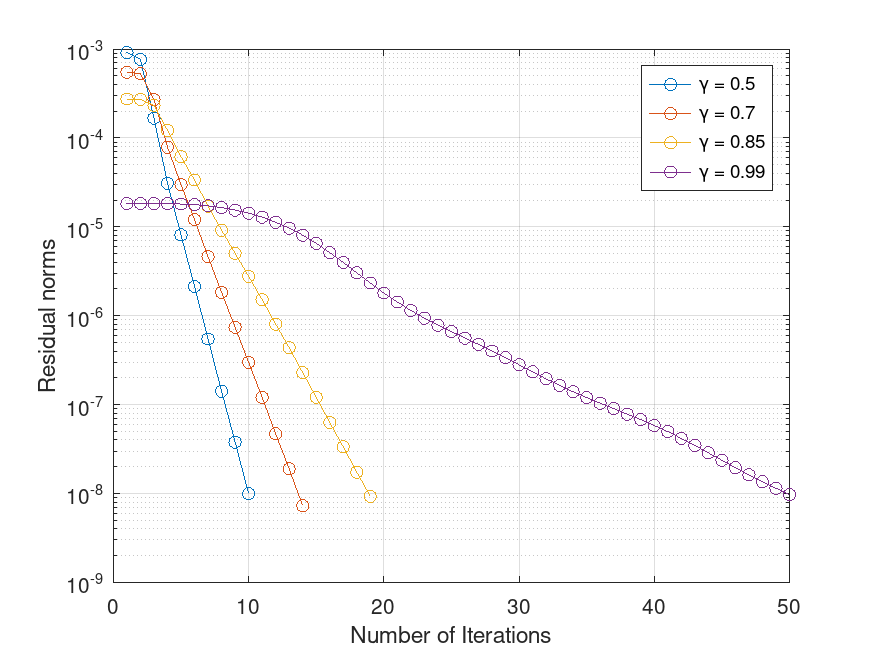
\includegraphics[width=0.7\textwidth]{convergence.png}
\caption{Convergence of GMRES for different values of $\gamma$.}
\label{fig:conv}
\end{figure}

\begin{thebibliography}{4}
\bibitem{bini}
Dario A. Bini (2019) \emph{Il Problema del PageRank}, appunti del corso di Calcolo Scientifico

\bibitem{notes}
Stefano Massei, Leonardo Robol (2023) \emph{Scientific Computing}, Lecture Notes
\end{thebibliography}
\end{document}
